
\documentclass[letterpaper,12pt,]{article}


\usepackage{titling}

\setlength{\droptitle}{5in}   % This is your set screw

\usepackage[%
    left=1in,%
    right=1in,%
    top=1in,%
    bottom=1.0in,%
    paperheight=11in,%
    paperwidth=8.5in%
]{geometry}%
\usepackage{comment}

\usepackage{listings}
\usepackage{graphicx}
\usepackage{amsmath}
\usepackage{amsmath}
\usepackage[section]{placeins}
\usepackage[font=small,skip=-2pt]{caption}
\usepackage{subcaption}
\usepackage{booktabs} % Tables
\usepackage{hyperref}
\usepackage{algorithm} 
\usepackage{algpseudocode}
\usepackage{pdflscape}

\lstdefinestyle{mystyle}{
    %backgroundcolor=\color{backcolour},   
    %commentstyle=\color{codegreen},
    %keywordstyle=\color{magenta},
    %numberstyle=\tiny\color{codegray},
    %stringstyle=\color{codepurple},
    basicstyle=\footnotesize,
    breakatwhitespace=false,         
    breaklines=true,                 
    captionpos=b,                    
    keepspaces=true,                 
    numbers=left,                    
    numberstyle=\footnotesize,               
    stepnumber=1,
    numbersep=5pt,
    showspaces=false,                
    showstringspaces=false,
    showtabs=false,                  
    tabsize=2,
    frame=single
}
\lstset{frame=single}

%\pagestyle{empty} % Remove page numbering
\linespread{1.5} % Line Spacing

\begin{document}
\begin{titlepage}

\newcommand{\HRule}{\rule{\linewidth}{0.5mm}} % Defines a new command for the horizontal lines, change thickness here

\center % Center everything on the page
 
%----------------------------------------------------------------------------------------
%	HEADING SECTIONS
%----------------------------------------------------------------------------------------


\textsc{\LARGE McGill University}\\[3.5cm]
\textsc{\Large Numerical Analysis}\\[0.5cm] 
\textsc{\large MATH 578}\\[2.5cm]

%----------------------------------------------------------------------------------------
%	TITLE SECTION
%----------------------------------------------------------------------------------------

{ \huge \bfseries Final Project}\\[1.5cm] % Title of your document

\HRule \\[0.4cm]
%----------------------------------------------------------------------------------------
%	AUTHOR SECTION
%----------------------------------------------------------------------------------------

\begin{minipage}{0.4\textwidth}
\begin{flushleft} \large
\emph{Name:}\\
Doug \textsc{Shi-Dong} % Your name
\end{flushleft}
\end{minipage}
~
\begin{minipage}{0.4\textwidth}
\begin{flushright} \large
\emph{Student ID:} \\
260466662\\
\end{flushright}
\end{minipage}\\[4cm]

\vfill{}
{\large December 14, 2015}\\[2cm]

\end{titlepage}


\section*{Problem Definition}

Given a structure and loads, the goal is to quickly evaluate stresses in real-time. For example, load sensors may be placed onto a helicopter and the pilot needs to know how close the structure is to failure. For ductile materials such as metals, von Mises stresses (or equivalent stresses) shown in Equation \ref{eq:3dvm} are usually used as the yield criterion.

\begin{equation}
\sigma_{VM} = \sqrt{\frac{1}{2}[
               (\sigma_{11}-\sigma_{22})^{2}
              +(\sigma_{22}-\sigma_{33})^{2}
              +(\sigma_{33}-\sigma_{11})^{2}
              +6(\sigma_{12}^2+\sigma_{22}^2+\sigma_{31}^2)
              ]}
\label{eq:3dvm}
\end{equation}


As it will be shown, it is possible to evaluate complex structural problems almost instantly by combining stored solutions of simple problems. Consequently, real-time stresses can be available to the operator for in-flight testing.


\section*{Theory}

A common tool for engineers is to evaluate the stresses throughout the structure using the finite element method (FEM) to solve for the solid mechanics boundary value problem (BVP). However, the time required to compute the stresses is too long for the results to be useful in-flight.

Large deformations that cause plastic deformation are already in a range that is undesired in most cases. This allows for the assumption that the model goes under small deformations. Furthermore, linear elastic constitutive behavior is assumed such that no failure, contact or yield occurs. With those assumptions, the elasticity field equations are linear.

As a consequence, the principle of superposition may be applied due to the linearity of the partial differential equations. The principle of superposition shown in Theorem \ref{th:pos} states that stresses are directly proportial to the loads applied to the solid. Additionally, the combination of multiple solutions is also a valid solution.

\newtheorem{theorem}{Theorem}
\begin{theorem}
If the set $(\boldsymbol{\sigma_{1}}, \boldsymbol{\epsilon_{1}})$ and $(\boldsymbol{\sigma_{2}}, \boldsymbol{\epsilon_{2}})$ are solutions to the linear BVPs with boundary conditions $\mathbf{f_{1}}$ and $\mathbf{f_{2}}$ respectively, then the set $\boldsymbol{(\sigma_{1}} + \alpha\boldsymbol{\sigma_{2}}, \boldsymbol\epsilon_{1}+\alpha\boldsymbol{\epsilon_{2}})$ is a solution to the BVP with boundary conditions $\mathbf{f_{1}} + \alpha \mathbf{f_{2}}$, where $\alpha$ is a scalar.
\label{th:pos}
\end{theorem}

Note that the normal and shear stresses are linear, but the von Mises stresses are not.

\section*{Methodology}

Using ANSYS Parametric Design Language (APDL), it is possible to write a script to programmatically solve different FEM problems. For simplicity, a 2D pinned-pinned beam is used to demonstrate the theory as shown in Figure \ref{fig:pdef}.

\begin{figure}[h]
\centering
\includegraphics[width=0.7\textwidth,angle=-90]{pdef002.eps}
\caption{Problem Setup}
\label{fig:pdef}
\end{figure}

The geometry is meshed with PLANE42 elements which is used as a plane element. The normal and shear stresses $\boldsymbol{\sigma_{11}}$, $\boldsymbol{\sigma_{22}}$, $\boldsymbol{\sigma_{12}}$ are calculated and stored for a load of $(F_x,F_y) = (1, 0)$ at a boundary node location. The stresses are calculated and stored again for a load of $(F_x,F_y) = (0, 1)$ at the same location. This is repeated until the solution for every unit load at every node location is computed and stored.

Note that it is not necessary to pre-process the stress calculations for every elements. Since the location of the sensors would be known beforehand, the stresses only need to be computed for loads at those locations.

Once every solution has been pre-processed, it is possible to quickly calculate the solution for any new problem by taking a linear combination of the stored solutions. Since a unit load has been used for the pre-processed data, the stored solution is simply multiplied by the load of the current problem. 

It is important to remember that the von Mises stresses are not linearly dependent on the loads. Therefore, the normal and shear stresses are calculated first, and the combined results are used to compute the von Mises stresses.

Algorithm 1 and 2 outline the process. Notice that only Algorithm 1 solves for BVP, while Algorithm 2 merely sums existing data.

\begin{algorithm}
\caption{Pre-processing Algorithm}\label{pproc}
\begin{algorithmic}[1]
\State \Call{CreateModel}{}
\State $F(1) \gets (1,0)$
\State $F(2) \gets (0,1)$
\For{$iloc \gets 1,nloc$} \Comment{Loop Over Locations of Interest}
\For{$ifor \gets 1,2$}
  \State \Call{Assign}{$F(ifor)$. $location(iloc)$}
  \State $\sigma(ifor,iloc) \gets $ \Call{SolveStresses}{} \Comment{Using APDL}
  \State \Call{StoreStresses}{$\sigma(ifor,iloc)$}
\EndFor
\EndFor
\end{algorithmic}
\end{algorithm}


\begin{algorithm}
\caption{Quick Von Mises Stress Evaluation Algorithm}\label{VMalg}
\begin{algorithmic}[1]
\State \Call {getLoads}{$F, nload$}
\State \Call {importStresses}{$\sigma$}

\State $s\gets 0$
\For{$iload \gets 1,nload$}
  \State $s \gets s + F(iload) * \sigma(iload)$ \Comment{Linear Combination}
\EndFor

\State $s_{vm} \gets $ \Call{evalVM}{s}

\State \Return max($s_{vm}$)

\end{algorithmic}
\end{algorithm}

\section*{Test Case}

Multiple loads are defined on the structure as shown in Figure \ref{fig:case1}. Figure \ref{fig:resxx1} and \ref{fig:res1} shows the computed solution by APDL, which fully matches the results from taking a linear combination. Table \ref{tab:lincomb} shows that taking the linear combination of the stored solutions give the same maximum stress $\sigma_{xx}$ of 22.4247 as solving the FEM model in Figure \ref{fig:resxx1}.

\begin{table}[h]
\centering
\begin{tabular}{r|rr|rr|r} \toprule
    {$N$} & {$F_x$} & {$\sigma_{1xx}(F = (1,0))$} & {$F_y$} & {$\sigma_{2xx}(F=(0,1))$} & {$F_x\sigma_{1xx}+F_y\sigma_{2xx}$}\\ \midrule
1 & -0.5 & -0.146913 & 0.0 & 0.269478 & 0.073457 \\
2 & -0.5 & -0.140176 & 0.0 & 0.269478 & 0.070088 \\
3 & -0.5 & -0.133439 & 0.0 & 0.269478 & 0.066720 \\
4 & -0.5 & -0.126702 & 0.0 & 0.269478 & 0.063351 \\
5 & -0.5 & -0.119965 & 0.0 & 0.269478 & 0.059983 \\
6 & -0.5 & -0.113229 & 0.0 & 0.269478 & 0.056614 \\
7 & -0.5 & -0.106492 & 0.0 & 0.269478 & 0.053246 \\
8 & -0.5 & -0.099755 & 0.0 & 0.269478 & 0.049877 \\
9 & -0.5 & -0.093018 & 0.0 & 0.269478 & 0.046509 \\
10 & -0.5 & -0.086281 & 0.0 & 0.269478 & 0.043140 \\
11 & -0.5 & -0.079544 & 0.0 & 0.269478 & 0.039772 \\
12 & 0.0 & -0.079544 & 1.0 & 0.202108 & 0.202108 \\
13 & 0.0 & -2.116161 & -2.0 & -10.799915 & 21.599831 \\
\bottomrule
\end{tabular}
\caption{Linear Combination of Stress $\sigma_{xx}$ at the Location of Maximum Stress}
\label{tab:lincomb}
\end{table}

\section*{Codes}

All codes are available on GitHub.

\url{https://github.com/dougshidong/math578/tree/master/Project}
\begin{landscape}
\newpage
\begin{figure}[h]
\centering
\includegraphics[width=1.0\textwidth,angle=-90]{tcase000.eps}
\caption{Test Case}
\label{fig:case1}
\end{figure}

\newpage
\begin{figure}[h]
\centering
\includegraphics[width=1.0\textwidth,angle=-90]{tcasesolxx.eps}
\caption{Solution $\sigma_{xx}$}
\label{fig:resxx1}
\end{figure}

\newpage
\begin{figure}[h]
\centering
\includegraphics[width=1.0\textwidth,angle=-90]{tcasesol.eps}
\caption{Solution $\sigma_{VM}$ Von Mises Stresses}
\label{fig:res1}
\end{figure}

\end{landscape}



\end{document}
